\documentclass[11pt,a4paper]{article}


%%% packages

  \usepackage{a4wide, tikz}


%%% TikZ

  \usetikzlibrary{calc}
  \tikzset{ v/.style = { circle
                       , draw
                       , thick
                       , inner sep    = 0.5pt
                       , minimum size = 6.0mm
                       },
            t/.style = { circle
            , draw = black
            , thick
            , inner sep    = 0.5pt
            , minimum size = 6.0mm
            }
          }



%%% front matter

  \title{Coursework 3}
  \author{Graph Algorithms and Complexity Theory}
  \date{Semester 1 Session 2019--2020}

\begin{document}

\maketitle
\thispagestyle{empty}

\noindent In the graph below a matching is indicated by bold lines. 
Execute \textsc{Edmonds}' algorithm starting from this matching. 
Give the alternating trees you grow as well as the graphs obtained by
shrinking blossoms.

\begin{center}
  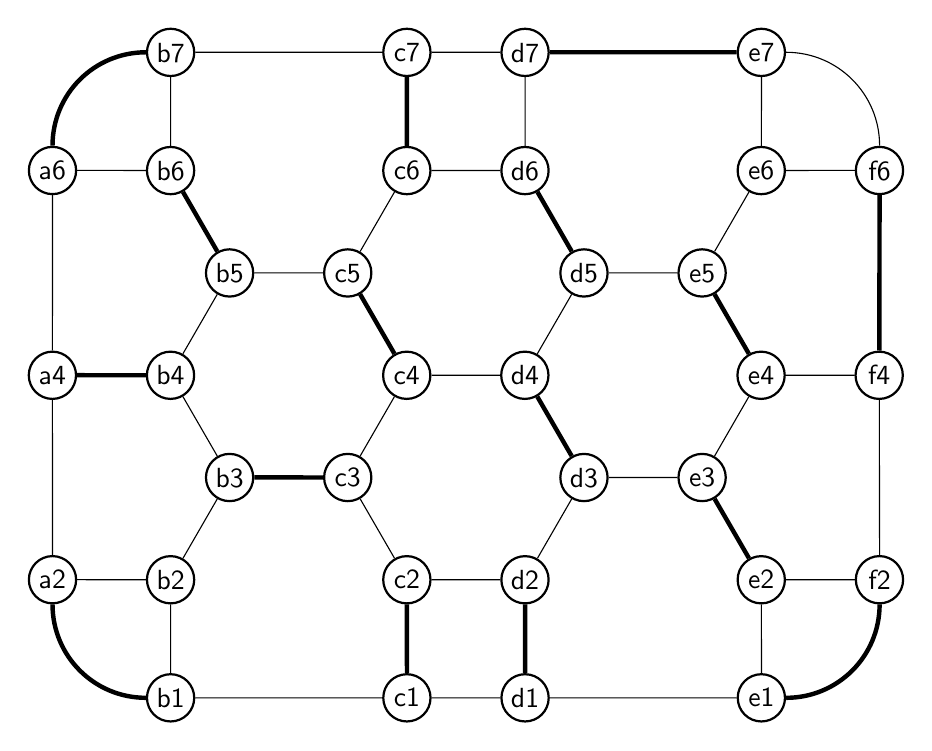
\begin{tikzpicture}[scale=1.5, bend angle=45, font=\sffamily]
    \foreach \n/\x in {a/1, b/2, c/4, d/5, e/7,f/8} {
      \node[v] (\n4) at (\x,4) {\n4};
    }
    \foreach \n in {b,d} {
      \node[v] (\n3) at ($(\n4) + (300:1)$) {\n3};
      \node[v] (\n5) at ($(\n4) + ( 60:1)$) {\n5};
      \node[v] (\n2) at ($(\n3) + (240:1)$) {\n2};
      \node[v] (\n6) at ($(\n5) + (120:1)$) {\n6};
      \node[v] (\n1) at ($(\n2) + (270:1)$) {\n1};
      \node[v] (\n7) at ($(\n6) + ( 90:1)$) {\n7};
    }
    \foreach \n in {c,e} {
      \node[v] (\n3) at ($(\n4) + (240:1)$) {\n3};
      \node[v] (\n5) at ($(\n4) + (120:1)$) {\n5};
      \node[v] (\n2) at ($(\n3) + (300:1)$) {\n2};
      \node[v] (\n6) at ($(\n5) + ( 60:1)$) {\n6};
      \node[v] (\n1) at ($(\n2) + (270:1)$) {\n1};
      \node[v] (\n7) at ($(\n6) + ( 90:1)$) {\n7};
    }
    \foreach \h in {2,6} {
      \node[v] (a\h) at ($(b\h) + (180:1)$) {a\h};
      \node[v] (f\h) at ($(e\h) + (  0:1)$) {f\h};
    }
    \draw[ultra thick] (a2) to[bend right] (b1)
                       (e1) to[bend right] (f2)
                       (b7) to[bend right] (a6);
    \draw[ultra thick] (c1)--(c2)  (d1)--(d2)  (b3)--(c3)  (e2)--(e3)
           (a4)--(b4)  (c4)--(c5)  (d3)--(d4)  (e4)--(e5)  (f4)--(f6)
           (b5)--(b6)  (c6)--(c7)  (d5)--(d6)  (d7)--(e7);
    \draw (f6) to[bend right] (e7);
    \draw (b2)--(b3)--(b4)--(b5)--(c5)--(c6)--(d6)--(d7)--(c7)--(b7)--(b6)
        --(a6)--(a4)--(a2)--(b2)--(b1)--(c1)--(d1)--(e1)--(e2)--(f2)--(f4)
        --(e4)--(e3)--(d3)--(d2)--(c2)--(c3)--(c4)--(d4)--(d5)--(e5)--(e6)
        --(f6)  (e6)--(e7);
  \end{tikzpicture}
\end{center}


\vspace{\fill}

\begin{center}
    \begin{minipage}{.35\textwidth}
        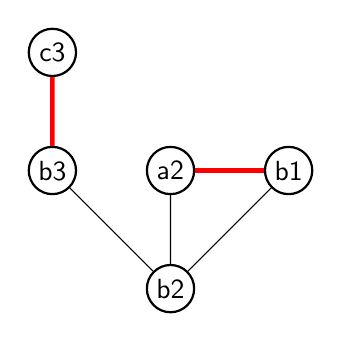
\begin{tikzpicture}[font=\sffamily]
            [level distance=10mm,
            % every node/.style={fill=red!60,circle,inner sep=1pt},
            %,nodes={fill=red!30}
            level 1/.style={sibling distance=15mm},
            level 2/.style={sibling distance=8mm},
            level 3/.style={sibling distance=11mm}]
            \node[t]  {b2} [grow=up]
            %[sibling distance=0.7cm,level distance = 1.4cm,red]
            child[draw=black, thin] { 
                node[t] (b1) {b1}
            }
            child [draw=black, thin] {
                node[t] (a2) {a2}
            }
            child [draw=black, thin] {
                node[t] {b3}
                child[draw=red, ultra thick] {
                    node[t] {c3}
                }
            };
            \path[draw=red,ultra thick] (b1) edge(a2);
            \end{tikzpicture}

    \end{minipage}
    \begin{minipage}{.35\textwidth}
        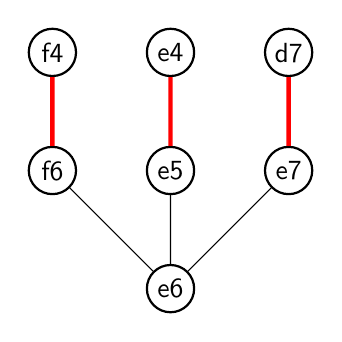
\begin{tikzpicture}[font=\sffamily]
            [level distance=10mm,
            % every node/.style={fill=red!60,circle,inner sep=1pt},
            %,nodes={fill=red!30}
            level 1/.style={sibling distance=15mm},
            level 2/.style={sibling distance=8mm},
            level 3/.style={sibling distance=11mm}]
            \node[t]  {e6} [grow=up]
            %[sibling distance=0.7cm,level distance = 1.4cm,red]
            child[draw=black, thin] { 
                node[t] (e7) {e7}
                child[draw=red, ultra thick] {
                    node[t] {d7}
                }
            }
            child [draw=black, thin] {
                node[t] (e5) {e5}
                child[draw=red, ultra thick] {
                    node[t] {e4}
                }
            }
            child [draw=black, thin] {
                node[t] {f6}
                child[draw=red, ultra thick] {
                    node[t] {f4}
                }
            };
        \end{tikzpicture}
    \end{minipage}
\end{center}

\hspace{\fill}

\begin{center}


    Reference:
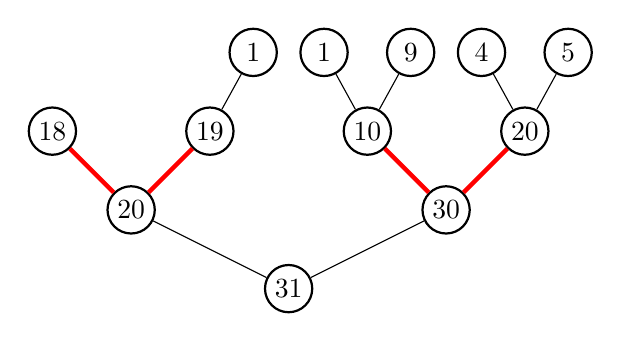
\begin{tikzpicture}
    [level distance=10mm,
    % every node/.style={fill=red!60,circle,inner sep=1pt},
    %,nodes={fill=red!30}
    level 1/.style={sibling distance=40mm},
    level 2/.style={sibling distance=20mm},
    level 3/.style={sibling distance=11mm}]
    \node[t]  {31} [grow=up]
    %[sibling distance=0.7cm,level distance = 1.4cm,red]
    child[draw=black, thin] { 
        node[t] {30}
        child[draw=red, ultra thick] { 
            node[t] {20}
            child[draw=black, thin] {
                node[t] {5}
                }
            child[draw=black, thin] {
                node[t] {4}
            }
        }
        child[draw=red, ultra thick] {
            node[t] {10}
            child[draw=black, thin] {
                node[t] {9}
                }
            child[draw=black, thin] {
                node[t] {1}
                }
            }
    }
    child [draw=black, thin] {
        node[t] {20}
        child[draw=red, ultra thick] {
            node[t] {19}
            child[draw=black, thin] {
                node[t] {1}
                }
            child[missing]
        }
        child[draw=red, ultra thick] {
            node[t] {18}
            }
    };
    \end{tikzpicture}

\end{center}

\begin{description}
    
\item[Submission:] Work out and present your solution on paper.
  Handwritten but legible is encouraged. Typeset and printed is fine
  too, but please do not use a copy machine.  Stitch together all your
  sheets and a filled header form and submit via SSO.  State on the
  header sheet which tutorial group you attend. The space to do so is
  the line ``Name of Lecturer Marking Work''.

    Since you will not receive a receipt for your submission, there is also
    the possibility to submit via Minerva. However, this is not required.
    A possible submission in Minerva will only be considered if your original
    paper submission gets lost.

  %% There are two options:
  %% \begin{description}
  %% \item[paper based:] Work out and present your solution on paper.
  %%   Handwritten but legible is encouraged, but please do not use a copy machine.
  %%   Stitch together all your sheets and a filled header form and submit via SSO.
  %%   A new letter box should appear soon.
  %% \item[digital:] Work out and present your solution in PDF.
  %%   \LaTeX\ is recommended, but any other text processor is fine too.
  %%   Submit via VLE.
  %% \end{description}

\item[Deadline:] Monday 18 November 2019, 10am.
  
\item[Credits:] This piece of summative coursework is worth 5\% of your grade.

\end{description}

\end{document}
